\section{Methodology}\label{sec:method}

This section describes the planned study design, the instrument, the
statistical methods and the validation of the analysis pipeline.
All symbols are collected in \autoref{tab:notation}.

\subsection{Design and Participants}\label{sec:design}
The study is cross-sectional: every teacher fills in the questionnaire once.
Two groups are compared, teachers of state schools and teachers of private
schools. The planned sample is 30--40 teachers in total (15--20 per group),
and a group is analysed only if it contains at least 15 respondents.
Participation is voluntary and anonymous.

\subsection{Instrument and Scoring}\label{sec:instrument}
Burnout is measured with the Maslach Burnout Inventory (MBI)
\cite{maslach1981mbi,maslach2001job} in the Russian-language adaptation of
Vodopyanova and Starchenkova~\cite{vodopyanova2008burnout}. The inventory has
three scales: emotional exhaustion (EE, 9 items), depersonalization (DP, 5
items) and reduced personal accomplishment (RPA, 8 items). Each item is
answered on a scale from 0 to 6, so the scale score is the sum of its items:
\begin{equation}
  S_k = \sum_{i \in I_k} x_i, \qquad k \in \{\mathrm{EE},\mathrm{DP},\mathrm{RPA}\},
  \label{eq:scale}
\end{equation}
where $I_k$ is the set of items of scale $k$ and $x_i$ is the answer to item
$i$. The scores range from 0 to 54 for EE, from 0 to 30 for DP and from 0 to
48 for RPA. To obtain one overall burnout index, each scale is standardised
over the sample and the three values are combined:
\begin{equation}
  B = z(S_{\mathrm{EE}}) + z(S_{\mathrm{DP}}) - z(S_{\mathrm{RPA}}),
  \qquad z(S) = \frac{S - \bar{S}}{s_S},
  \label{eq:index}
\end{equation}
where $\bar{S}$ and $s_S$ are the sample mean and standard deviation of the
scale score. The sign of $z(S_{\mathrm{RPA}})$ is negative because a high
value on this scale means a high personal accomplishment, that is, less burnout.

\subsection{Reliability}\label{sec:reliability}
The internal consistency of each scale is checked with Cronbach's
$\alpha$~\cite{cronbach1951alpha}:
\begin{equation}
  \alpha = \frac{m}{m-1}\left(1 - \frac{\sum_{i=1}^{m}\sigma_i^{2}}{\sigma_{T}^{2}}\right),
  \label{eq:alpha}
\end{equation}
where $m$ is the number of items in the scale, $\sigma_i^2$ is the variance of
item $i$ and $\sigma_T^2$ is the variance of the scale score. A scale is
accepted as reliable if $\alpha \ge 0.7$.

\subsection{Group Comparison}\label{sec:tests}
The main comparison (RQ1) is the difference in emotional exhaustion between the
two groups. For group means $\bar{x}_1,\bar{x}_2$, standard deviations
$s_1,s_2$ and sizes $n_1,n_2$, we use Welch's $t$-test~\cite{welch1947t}, which
does not assume equal variances:
\begin{equation}
  t = \frac{\bar{x}_1 - \bar{x}_2}{\sqrt{s_1^{2}/n_1 + s_2^{2}/n_2}}.
  \label{eq:welch}
\end{equation}
The size of the difference is reported as Cohen's $d$:
\begin{equation}
  d = \frac{\bar{x}_1 - \bar{x}_2}{s_p},
  \qquad
  s_p = \sqrt{\frac{(n_1-1)s_1^{2} + (n_2-1)s_2^{2}}{n_1+n_2-2}}.
  \label{eq:cohen}
\end{equation}
Because of the small groups, the Mann--Whitney test~\cite{mann1947u} is
computed as a robustness check, and the uncertainty of the estimates is shown
with percentile-bootstrap confidence intervals~\cite{efron1979bootstrap}.
All tests are two-tailed with significance level $\alpha_{\mathrm{test}}=0.05$.
RQ2 repeats the comparison for each scale separately, and RQ3 is exploratory
(Spearman correlations and hierarchical regression in JASP).

\subsection{Pipeline Validation}\label{sec:pipeline}
The analysis is run by a Python pipeline in a pinned Docker image with a fixed
random seed (42). To show that the pipeline is fast enough to be re-run after
every data update, we measured it on synthetic questionnaires with
$n \in \{35,100,1000\}$ respondents. For a run $r$ with workload $n$ and
duration $\ell$, the throughput and the scaling relative to the baseline
$n_0=35$ are
\begin{equation}
  \theta = \frac{n}{\ell},
  \qquad
  S(n) = \frac{\theta(n)}{\theta(n_0)},
  \qquad
  E(n) = \frac{S(n)}{n/n_0}.
  \label{eq:speedup}
\end{equation}
Each workload was run 40 times after 10 discarded warm-up runs, and the
latency percentiles are reported with 95\,\% bootstrap intervals
($B=10\,000$ resamples). The setup is summarised in \autoref{tab:params}; the
measured latency and throughput are shown in \autoref{fig:pipeline}.
The measurements concern only the software and contain no information about
teachers.

\begin{table}[t]
  \centering
  \caption{Notation used in \autoref{eq:scale}--\autoref{eq:speedup}.}
  \label{tab:notation}
  \small
  \begin{tabular}{@{}ll@{}}
    \toprule
    Symbol & Meaning \\
    \midrule
    $S_k$ & sum score of scale $k$ (EE, DP, RPA) \\
    $z(\cdot)$ & standardised score \\
    $B$ & overall burnout index \\
    $\alpha$ & Cronbach's alpha \\
    $t$, $d$ & Welch statistic, Cohen's effect size \\
    $\theta$, $S$, $E$ & throughput, speed-up, efficiency \\
    \bottomrule
  \end{tabular}
\end{table}

\begin{table}[t]
  \centering
  \caption{Parameters of the study and of the pipeline validation.}
  \label{tab:params}
  \small
  \begin{tabular}{@{}lr@{}}
    \toprule
    Parameter & Value \\
    \midrule
    Planned sample (teachers) & 30--40 \\
    Minimum per group & 15 \\
    Significance level & 0.05 \\
    Reliability threshold $\alpha$ & 0.7 \\
    Random seed & 42 \\
    Workloads $n$ & 35, 100, 1000 \\
    Measured runs per $n$ & 40 \\
    Warm-up runs & 10 \\
    Bootstrap resamples $B$ & 10\,000 \\
    \bottomrule
  \end{tabular}
\end{table}

\begin{figure*}[t]
  \centering
  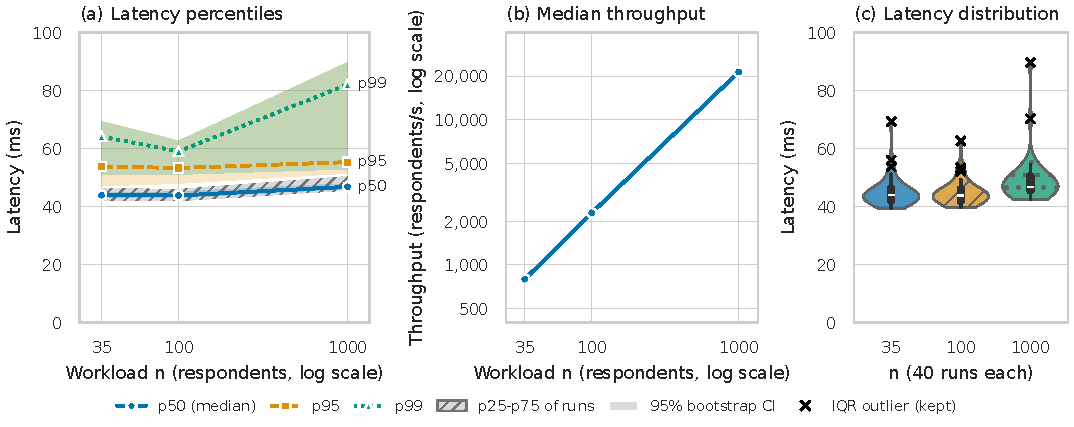
\includegraphics[width=\textwidth]{fig_combined_latency_throughput.pdf}
  \caption{Pipeline validation on synthetic data: (a)~latency percentiles,
  (b)~median throughput, (c)~distribution of run latency for
  $n=35$, $100$, $1000$ respondents (40 runs each). Bands are 95\,\%
  bootstrap intervals. Median latency stays between 43.8 and 46.8\,ms while
  throughput grows from 797 to 21\,371 respondents/s.}
  \label{fig:pipeline}
\end{figure*}
